\subsubsection{Giới thiệu bộ dữ liệu}
    \paragraph{Nguồn dữ liệu}
    \leavevmode

    Bộ dữ liệu là bộ dữ liệu hình ảnh X-quang ngực được gán nhãn nhằm hỗ trợ phát hiện COVID-19, bởi Hội Tin học Hình ảnh trong Y học (Society for Imaging Informatics in Medicine - SIIM) hợp tác với Quỹ thúc đẩy nghiên cứu y sinh và sức khỏe của khu vực Valencia (Foundation for the Promotion of Health and Biomedical Research of Valencia Region - FISABIO) và Hiệp hội X quang Bắc Mỹ (Radiological Society of North America - RSNA)

    \paragraph{Mô tả dữ liệu}
    \leavevmode
    
    Bộ dữ liệu bao gồm 6,334 hình ảnh X-quang kích thước 256x256 kèm file gắn nhãn. Các hình ảnh được gán nhãn khung vùng lạ, hoặc không có nếu không có phát hiện lạ.

    Ví dụ một phần dữ liệu:

    \begin{figure}[htp]
        \centering
        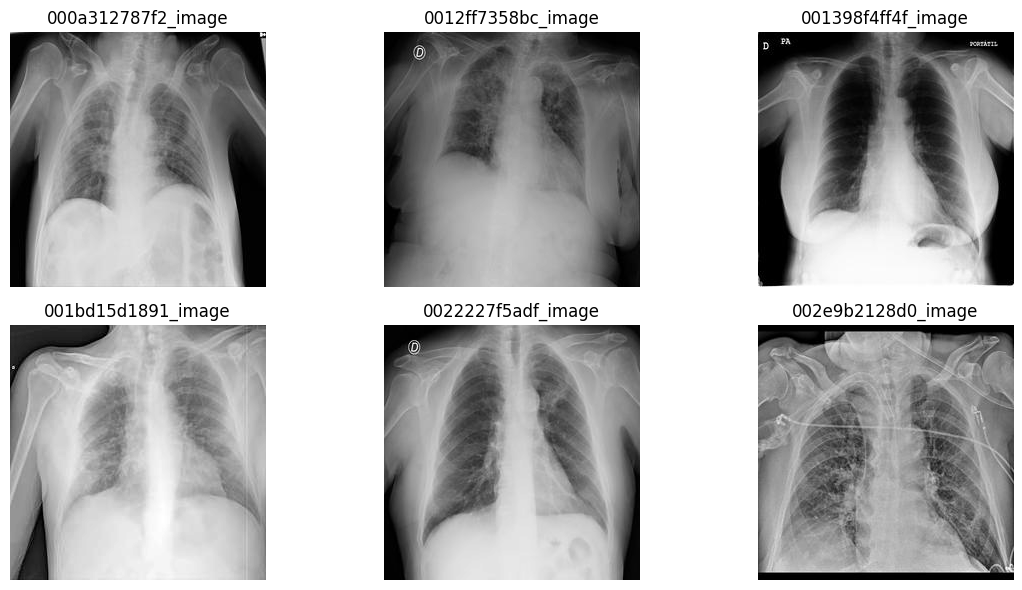
\includegraphics[width=0.90\textwidth]{images/Img_lung_label1_exp.png}
        \caption{Hình ảnh X-quang có phát hiện vùng lạ}
        \label{fig:Img_lung_label1_exp}
    \end{figure}
    \FloatBarrier

    \begin{figure}[htp]
        \centering
        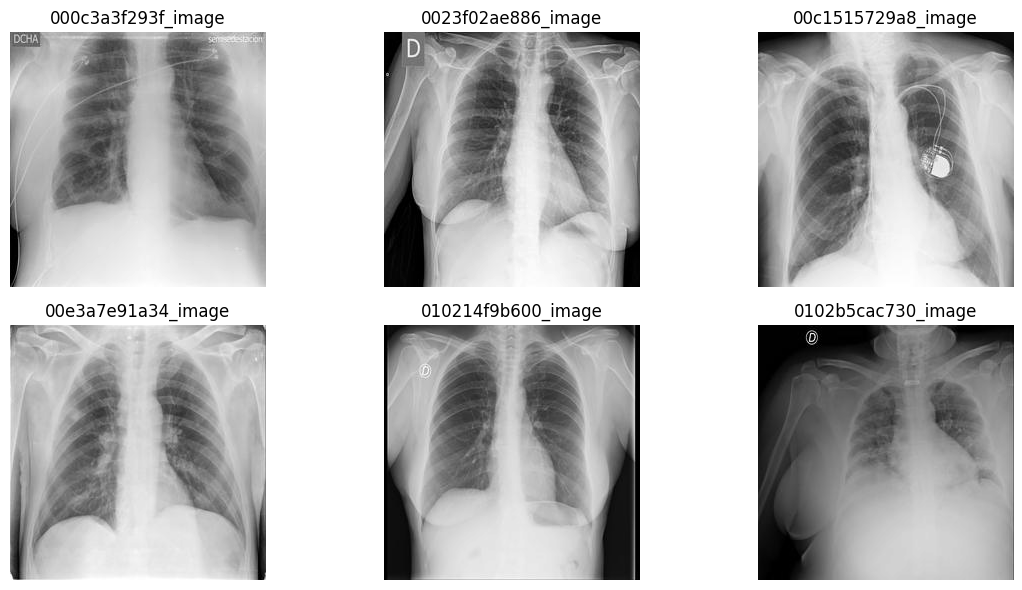
\includegraphics[width=0.90\textwidth]{images/Img_lung_label0_exp.png}
        \caption{Hình ảnh X-quang không phát hiện vùng lạ}
        \label{fig:Img_lung_label0_exp}
    \end{figure}
    \FloatBarrier

\subsubsection{Phân tích, trực quan hóa dữ liệu}
   

    \begin{figure}[htp]
        \centering
        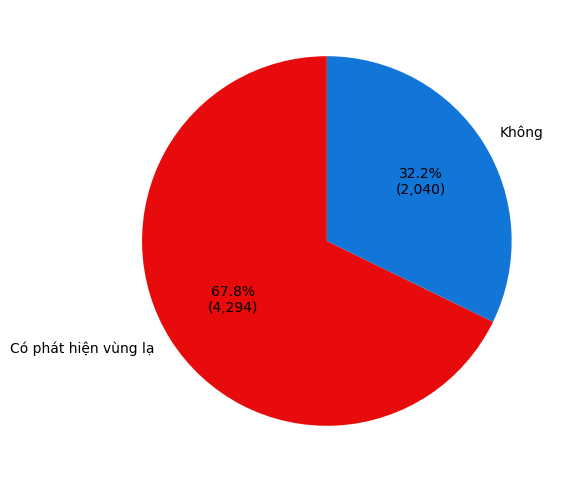
\includegraphics[width=0.50\textwidth]{images/Img_lung_label.png}
        \caption{Số lượng hình ảnh mỗi nhãn}
        \label{fig:Img_lung_label}
    \end{figure}
    \FloatBarrier

    Biểu đồ pie \ref{fig:Img_lung_label} cho thấy sự phân phối dữ liệu giữa hai nhãn. Dữ liệu mất cân bằng với số lượng hình có phát hiện vùng lạ chiếm đến 67.8\% tập dữ liệu.

    \begin{figure}[htp]
        \centering
        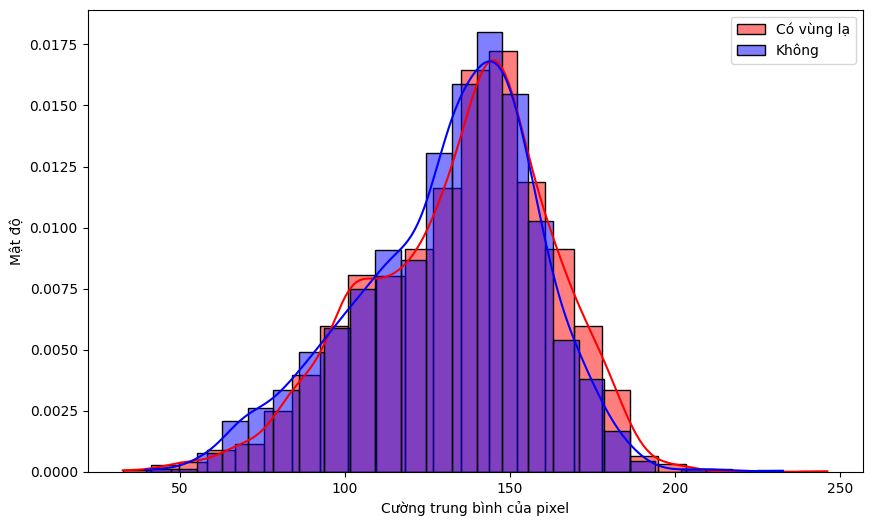
\includegraphics[width=0.90\textwidth]{images/Img_lung_intensity.png}
        \caption{Phân phối cường độ pixel trung bình}
        \label{fig:Img_lung_intensity}
    \end{figure}
    \FloatBarrier

    Biểu đồ \ref{fig:Img_lung_intensity} cho thấy sự phân phối cường độ pixel trung bình giữa hai nhóm ảnh. Cả hai phân phối đều có hình chuông và khá giống nhau. Nhóm ảnh có cùng lạ hơi lệch về cường độ cao hơn một ít, tuy nhiên đó là không đáng kể.

    \begin{figure}[htp]
        \centering
        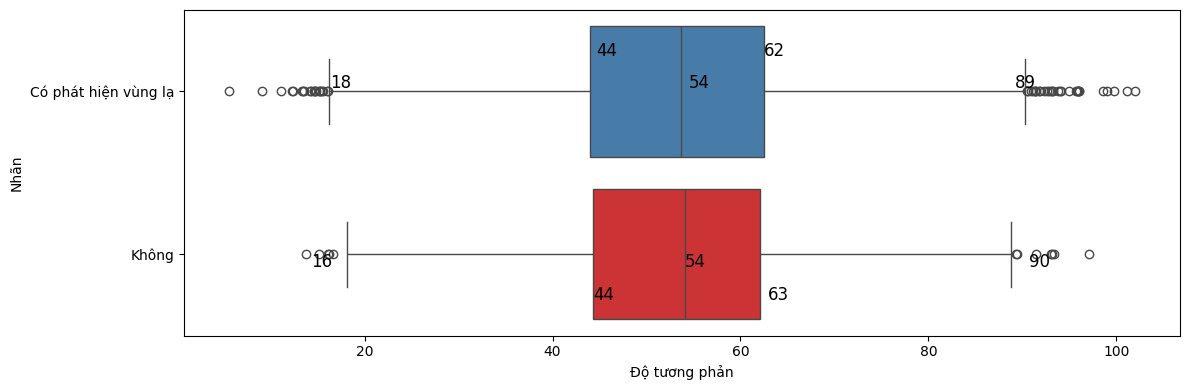
\includegraphics[width=0.90\textwidth]{images/Img_lung_contrast.png}
        \caption{Độ tương phản theo nhãn}
        \label{fig:Img_lung_contrast}
    \end{figure}
    \FloatBarrier

     Biểu đồ \ref{fig:Img_lung_contrast} cho thấy độ tương phản giữa hai loại hình là tương đương nhau, với một số ngoại lệ.

     \begin{figure}[htp]
        \centering
        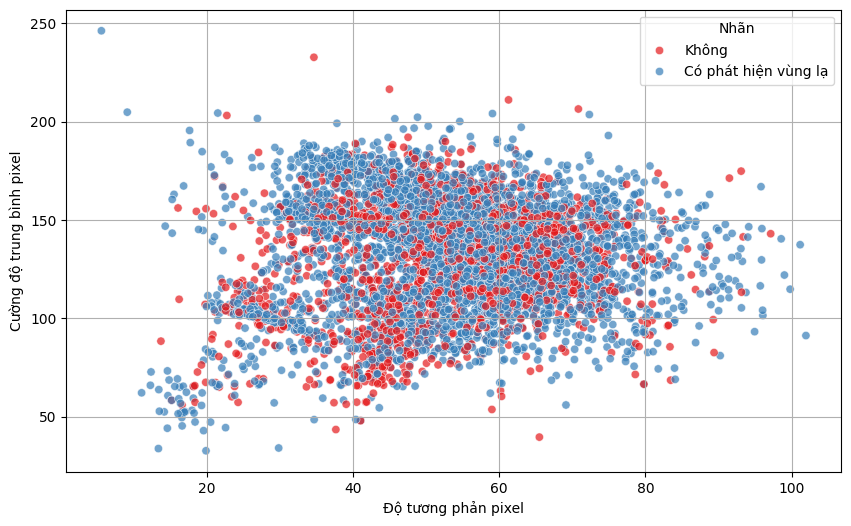
\includegraphics[width=0.90\textwidth]{images/Img_lung_intensity_contrast.png}
        \caption{Tương quan cường độ và tương phản pixel với loại nhãn}
        \label{fig:Img_lung_intensity_contrast}
    \end{figure}
    \FloatBarrier

    Biểu đồ \ref{fig:Img_lung_intensity_contrast} thể hiện mối quan hệ giữa độ tương phản pixel và cường độ trung bình pixel trên hai nhãn dữ liệu. Các điểm giữa hai nhãn không tạo ra phân vùng rõ rệt. 

\subsubsection{Mô hình hóa dữ liệu}
    Để thực hiện bài toán phân cụm, nhóm sử dụng đặc trưng được tính bằng cách chia ảnh thành các ô vuông nhỏ (patch) có kích thước cố định, sử dụng trung bình độ sáng của mỗi ô để tạo thành một vector đặc trưng.

    \paragraph{Phân cụm sử dụng K-means}
    \leavevmode

    \begin{figure}[htp]
        \centering
        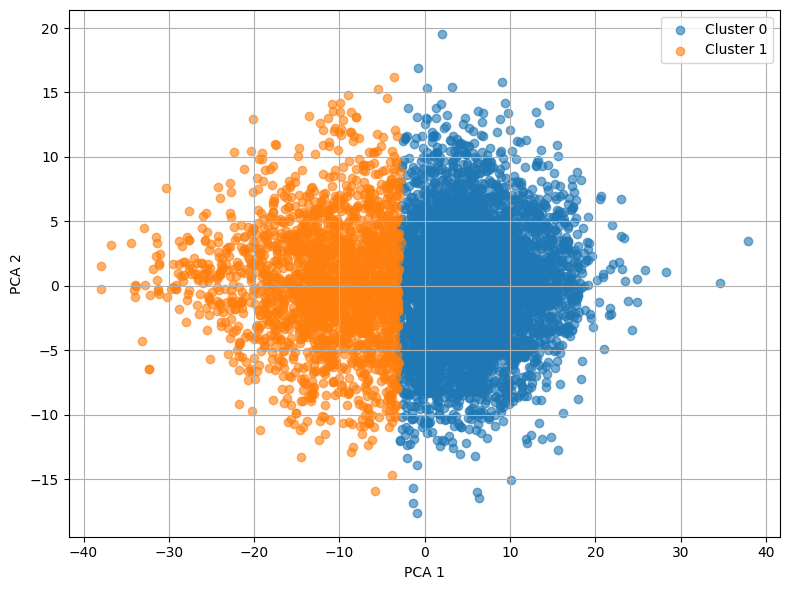
\includegraphics[width=0.90\textwidth]{images/Img_lung_kmeans.png}
        \caption{K-Means. ARI = 0.0039}
        \label{fig:Img_lung_kmeans}
    \end{figure}
    \FloatBarrier

    Biểu đồ \ref{fig:Img_lung_kmeans} cho thấy kết quả phân cụm ảnh X-quang ngực bằng thuật toán K-means, sử dụng giảm chiều dữ liệu bằng PCA để vẽ trên 2 chiều. Hai cụm được phân tách khá rõ ràng theo chiều ngang. Các điểm dữ liệu trong mỗi cụm khá tập trung và ít bị lẫn với cụm còn lại, cho thấy mô hình đã chia cụm ổn định về mặt hình ảnh. Giá trị ARI chỉ đạt 0.0039, cho thấy kết quả phân cụm gần như không tương quan với nhãn thực tế và hiệu quả phân cụm rất thấp.

    \paragraph{Phân cụm sử dụng Spectral Clustering}
    \leavevmode

    \begin{figure}[htp]
        \centering
        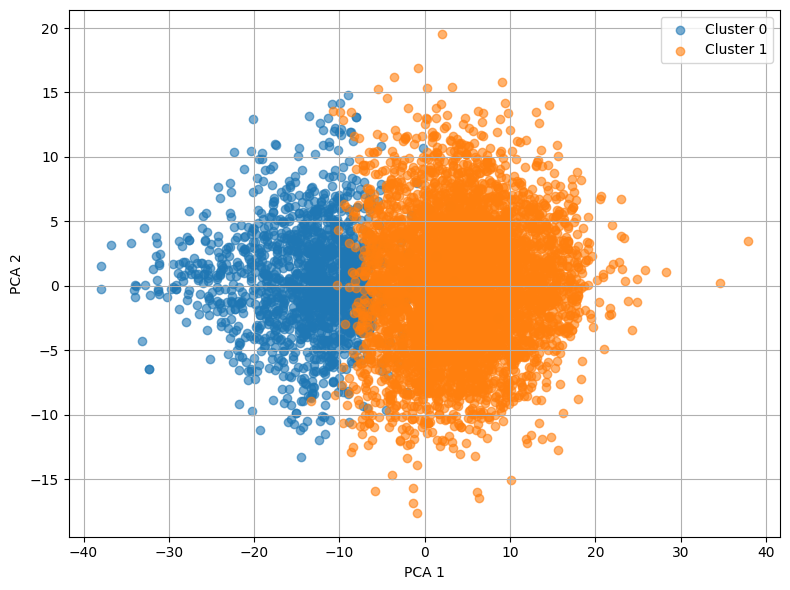
\includegraphics[width=0.90\textwidth]{images/Img_lung_spectral.png}
        \caption{Spectral Clustering. ARI = 0.0046}
        \label{fig:Img_lung_spectral}
    \end{figure}
    \FloatBarrier

    Biểu đồ \ref{fig:Img_lung_spectral} thể hiện kết quả phân cụm ảnh X-quang ngực bằng thuật toán Spectral Clustering sau khi giảm chiều dữ liệu bằng PCA. Các điểm dữ liệu phân bố hai cụm khá đều, nhưng có một số vùng chồng lấn nhẹ ở khu vực trung tâm. Mặc dù hình ảnh cho thấy một sự phân cụm tương đối rõ. ARI chỉ đạt 0.0046, cho thấy kết quả phân cụm chưa tốt, gần như ngẫu nhiên.

    \paragraph{Phân cụm sử dụng Gaussian Mixture}
    \leavevmode
    
    \begin{figure}[htp]
        \centering
        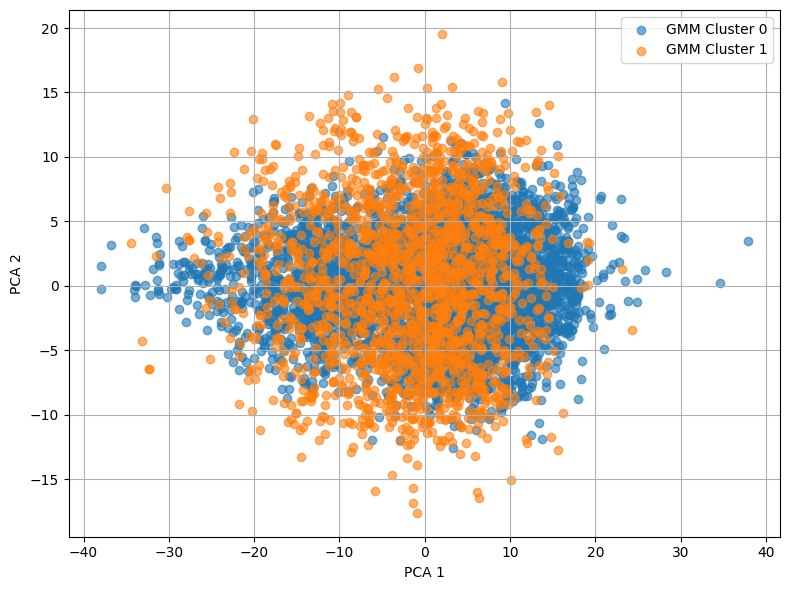
\includegraphics[width=0.90\textwidth]{images/Img_lung_gauss.png}
        \caption{Gaussian Mixture. ARI = -0.0095}
        \label{fig:Img_lung_gauss}
    \end{figure}
    \FloatBarrier

    Biểu đồ thể hiện kết quả phân cụm ảnh X-quang ngực bằng mô hình Gaussian Mixture (GMM) sau khi giảm chiều dữ liệu bằng PCA. Mô hình chia dữ liệu thành 2 cụm đè lên nhau. Chỉ số ARI = -0.0095 cho thấy kết quả phân cụm gần như hoàn toàn không tương quan với nhãn thực tế, thậm chí kém hơn cả phân cụm ngẫu nhiên.

    So sách các mô hình:

    \begin{table}[htbp]
        \centering
        \caption{So sánh kết quả các mô hình}
        \label{tab:lung-clustering-compare}
        \begin{tabular}{|l|c|}
        \hline
         Model & ARI  \\
        \hline
        K-Means & 0.0039  \\
        \hline
        Spectral Clustering & \textbf{0.0046} \\
        \hline
        Gaussian Mixture & -0.0095  \\
        \hline
        \end{tabular}
    \end{table}

    \FloatBarrier

    Bảng \ref{tab:lung-clustering-compare} so sánh cho thấy các mô hình phân cụm đều cho kết quả rất thấp, phản ánh khả năng phân tách các cụm gần như không đáng kể. Trong đó, Spectral Clustering đạt chỉ số ARI cao nhất với giá trị 0.0046, nhưng chênh lệch so với K-Means (0.0039) là không đáng kể. Mô hình Gaussian Mixture thậm chí còn cho kết quả âm (-0.0095), cho thấy việc phân cụm của nó còn tệ hơn ngẫu nhiên. Nhìn chung, cả ba mô hình đều không phù hợp để phân tách dữ liệu trong trường hợp này.
    

    